\subsection{Энергетические зависимости. \\Оптимальный набор параметров}

Для дальнейшего изучения системы с прикладной точки зрения имеет смысл поиск так называемого оптимума системы -- в нашем случае оптимального набора параметров и условий, при которых обеспечивается наилучшее (самое эффективное) излучение -- то есть мы должны стремиться к максимально эффективному преобразованию энергии, запасенной в остаточном токе, в энергию электромагнитного излучения заданной системы. 

Стоит также объяснить прикладной смысл и соответствующие выкладки данной работы. В реальных исследуемых моделях (конструкциях) подобный тип излучения достигается с помощью мощного короткого ионизирующего лазерного импульса, когда за несколько фемтосекунд ( $\sim10^{-15}$ сек) система из газа трансформируется в плазму (то есть происходит ионизация), при этом длительность этого импульса настолько мала, что электроны, ионы и нейтральные частицы не успевают существенно изменить свои положения в системе. То есть ионизированная система приобретает начальный импульс, который мы в уравнениях записываем как начальные условия, а уже после этого <<удара>> система начинает определенным образом эволюционировать и эту эволюцию мы и изучаем в данной работе. Ввиду таких коротких по времени возбуждениях системы, а также ввиду того, что размер системы много больше дебаевского радиуса, мы пренебрегаем температурным воздействием системы на саму себя. В данной работе это выражается в том, что уравнение для плотности тока в (\ref{eq:sys:start}) не содержит в себе прямую зависимость от температуры.

Конструкция полученной системы зависит как от типа, характера <<заряжающего>> импульса, так и от идеализации самой модели и выводов из неё, и прочих возможных допущениях, которые могут приниматься в зависимости от поставленной задачи. С изменением структуры системы, при изменении относительных размеров области спадающей границей по сравнению с участком плато наблюдается изменение колебательных свойств системы \cite{Vved2005}. Как уже говорилось выше, когда $\delta,\:\nu\rightarrow0$, то есть область неоднородности плазмы очень мала, система  имеет только одну резонансную частоту $\omega_{\text{рез}}=\omega_{p 0}/\sqrt{2}$, так называемую <<частоту геометрического резонанса>> \cite{Gilden2000}, которую можно обнаружить и с помощью данного вычислительного кода (рис. \ref{pic:spm_res}). С уменьшением частоты соударений спектр должен сужаться в пределе до дельта-функции в точке геометрического резонанса, а с увеличением, соответственно, расширяться.

\begin{figure}[H]\centering	
	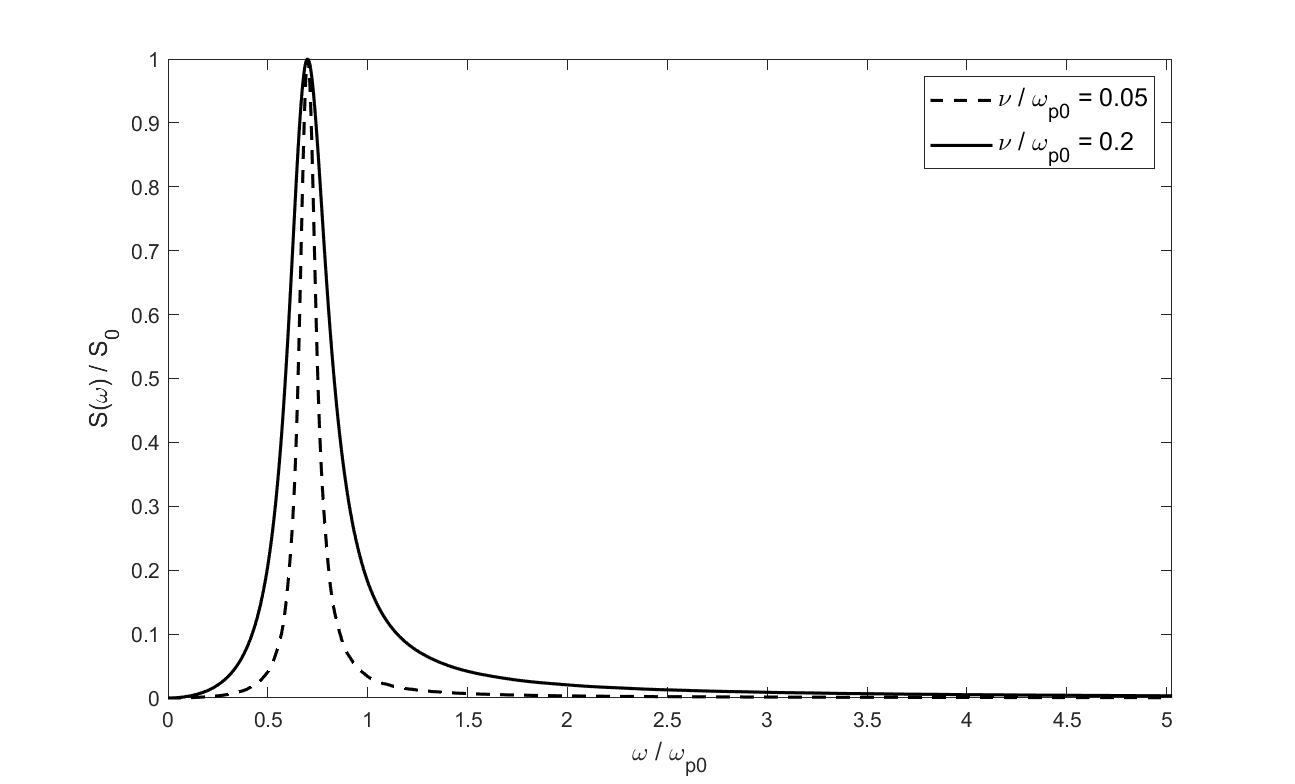
\includegraphics[scale=0.7]{pics/SPM_minimal}
	\caption{Наблюдение геометрического резонанса при $\delta=0.1, R_{2}=0.2,$  и различных значениях \\ $\nu/\omega_{p0} $ $(0.05$ и $0.2)$.}
	\label{pic:spm_res}
\end{figure}

Когда же область спадания приобретает определенный -- отличный от бесконечно малого -- размер, так как плазменная частота спадает от своего максимального значения до нуля, в этой области мы можем <<дойти>> до частоты, совпадающей с $\omega_{p 0}/\sqrt{2}$. Ввиду того, что распределение плазменной концентрации, а значит и $\omega_{p}$, не изменяется от времени, а их распределение от $r$ задано по \eqref{eq:N(r)}, $\omega_{\text{рез}}=\omega_{p 0}/\sqrt{2}$ ровно посередине области переменной концентрации (то есть, при $r=\frac{R_{1}+R_{2}}{2}$). Возникающий в данном случае эффект, когда плазменная частота совпадает с резонансной частотой, называется \textit{плазменный резонансом}. 

Возникновение плазменного резонанса порождает соответствующие энергетические потери в исследуемом объекте, причем если некоторые из возможных в данной задаче потерь всё же можно назвать полезными (например, потери радиационные -- то есть энергия теряется на излучении системы -- в их нахождении и эффективности основная суть данной работы) которые увеличивают эффективность моделируемого плазменного излучателя, а потери на соударении электронов с тяжелыми частицами можно сравнить с потерями энергии колебательных систем на затухании, то потери на резонансе --  естественно, являются потерями негативными -- однако, они напрямую зависят от ширины области неоднородной плотности плазмы, то есть от параметра $\delta$. Потери на соударении присутствуют в любой системе, где частота соударений $\nu$ ненулевая. Потери на излучении зависят от размеров системы, то есть от параметра $R_{2}$, и скорее связаны с её внутренними свойствами и способностями эффективно отдавать энергию, запасенную в остаточном токе. Подбор оптимальных параметров системы, когда энергия запасена в достаточном количестве, чтобы не поглотиться на резонансе и/или соударении, но при этом излученная энергия составляла бы б\'ольшую часть от запасенной, является основной задачей данной работы. Чем больше $\delta$, тем больше потери на резонансе преобладают над остальными потерями, что показывают расчеты на рисунке \ref{ris:kpd_r2_delta_07_1}.

Полученные расчеты поставленной задачи с множеством параметров, а также последующий расчет коэффициента полезного действия по формуле \eqref{eq:kpd_last} изображены на рисунке \ref{ris:kpd_delta_r2} (а, б).

\begin{figure}[H]	
	\begin{minipage}[H]{0.5\linewidth}
		\center{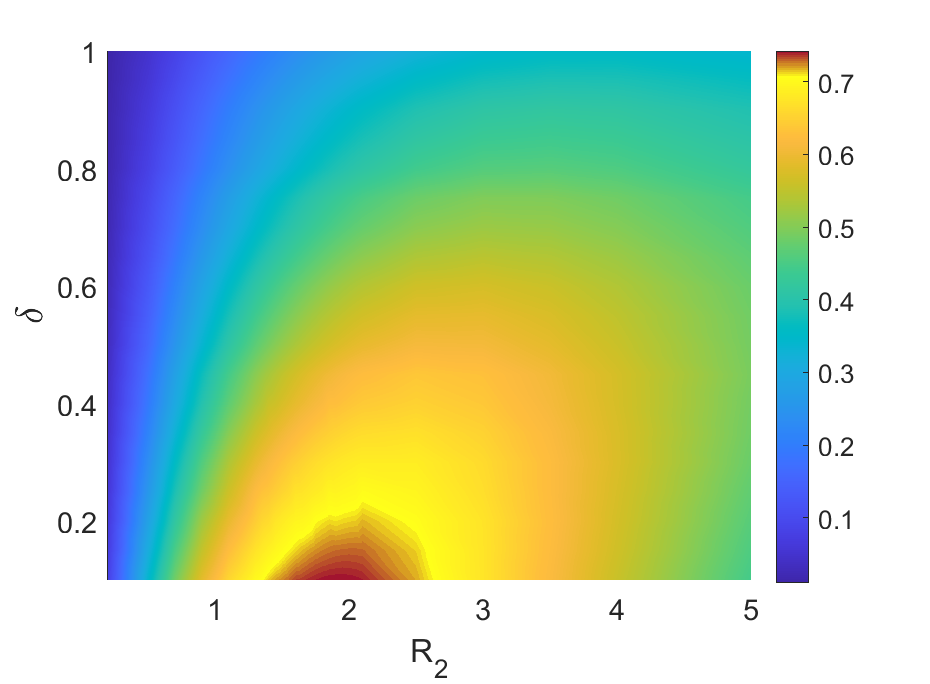
\includegraphics[width=1\linewidth]{pics/KPD_01} \\ а)}
	\end{minipage}	
	\begin{minipage}[H]{0.5\linewidth}
		\center{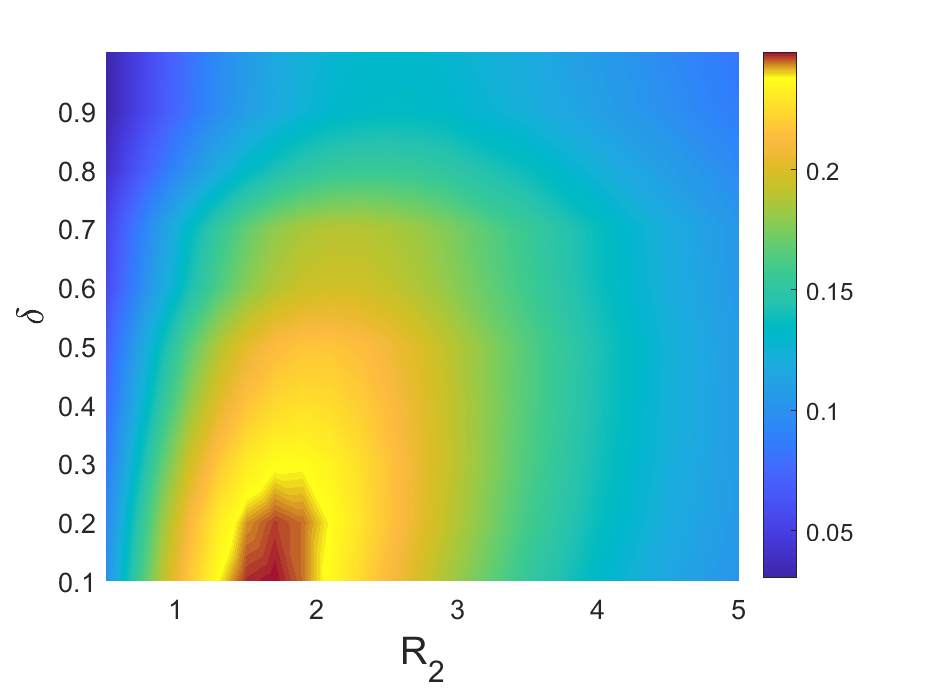
\includegraphics[width=1\linewidth]{pics/KPD_07} \\ б)}
	\end{minipage}
	\caption{Эффективность преобразования энергии, запасенной в остаточном токе в электромагнитную энергию излучения  в зависимости от радиуса цилиндра $R_{2}$ и размера неоднородной области  $\delta$ при  $\nu / \omega_{p 0}=0.1$ (а) и  $\nu / \omega_{p 0}=0.7$.}
	\label{ris:kpd_delta_r2}
\end{figure}
\newpage
Из полученных данных можно определить зону оптимальных значений $R_{2}$ и $\delta$ -- при которых КПД максимальный, то есть б\'ольшая часть энергии не переходит в негативные для нас потери, а излучается, то есть радиационные потери больше прочих. Также имеет смысл построить в оптимуме системы графики КПД от значений одного параметра при фиксированном значении другого и наоборот (рисунки \ref{ris:kpd_r2_delta_07} и \ref{ris:kpd_r2_delta_07_1}).

\begin{figure}[H]
	\centering
	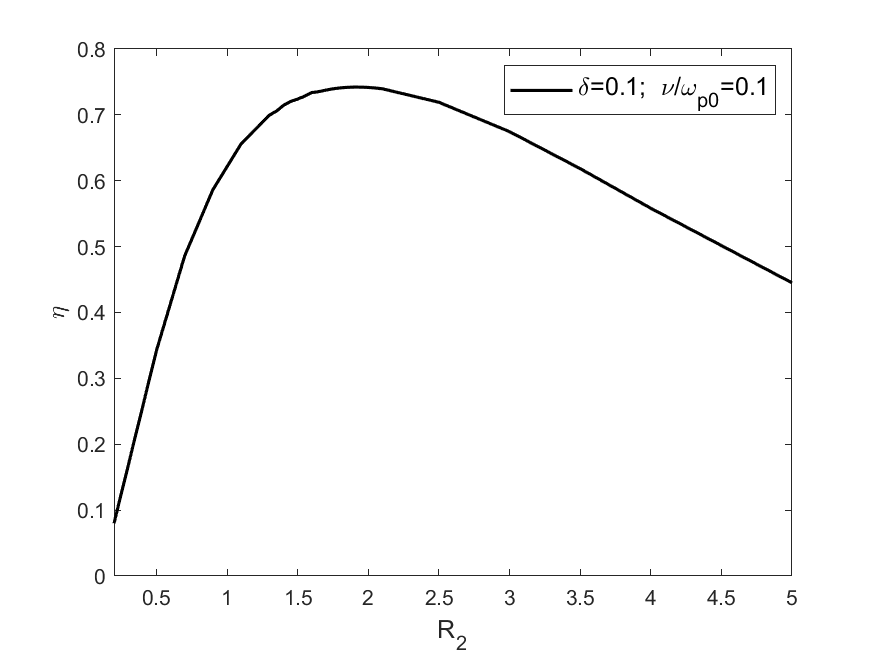
\includegraphics[scale=0.7]{pics/KPD_r2}
	\caption{Эффективность излучения при оптимальном размере неоднородной области $\delta=0.1$ в зависимости то радиуса цилиндра $R_{2}$ ($\nu / \omega_{p 0}=0.1$).}
	\label{ris:kpd_r2_delta_07}
\end{figure}

\begin{figure}[H]
	\centering
	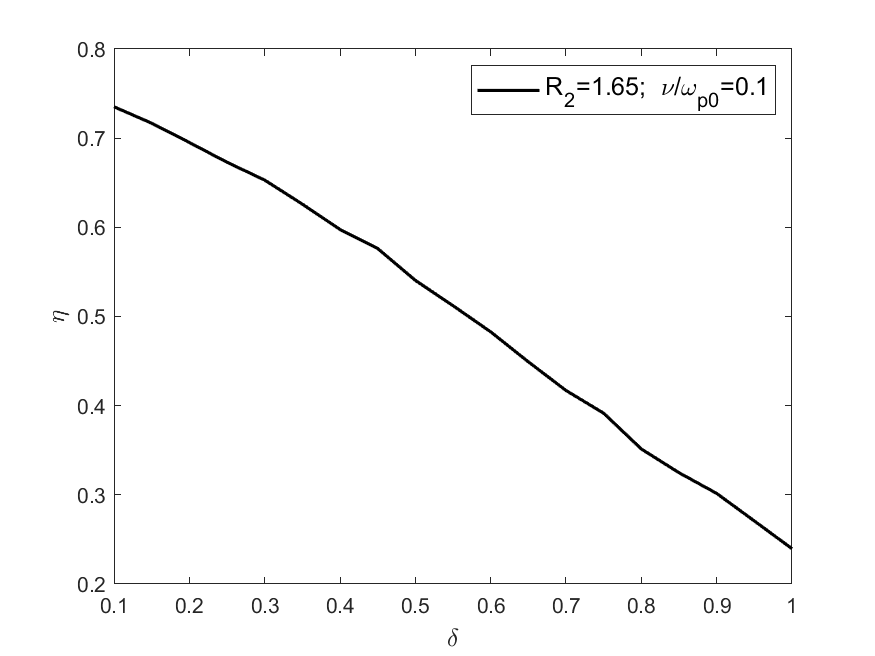
\includegraphics[scale=0.7]{pics/KPD_delta}
	\caption{Эффективность излучения при оптимальном радиусе цилиндра $R_{2}=1.64$ в зависимости от размера неоднородной области $\delta$. ($\nu / \omega_{p 0}=0.1$).}
	\label{ris:kpd_r2_delta_07_1}
\end{figure}


\newpage
Графики зависимостей КПД от нормированной частоты соударений при двух фиксированных $\delta$, что объясняет две различные ситуации, когда зона спада плазменной плотности либо мала по сравнению с общими размерами цилиндра $\left(\delta=0.1\right)$, либо составляет основную часть $\left(\delta=1\right)$, расположены на рисунке \ref{ris:kpd_nu}. Полученный рисунок объясняет, что эффективная излучаемая энергия системы падает при увеличении количества соударений в ней, то есть вместо резонансных потерь доминировать начинают уже потери на соударениях.

\begin{figure}[H]\centering
	\captionsetup{justification=centering}
	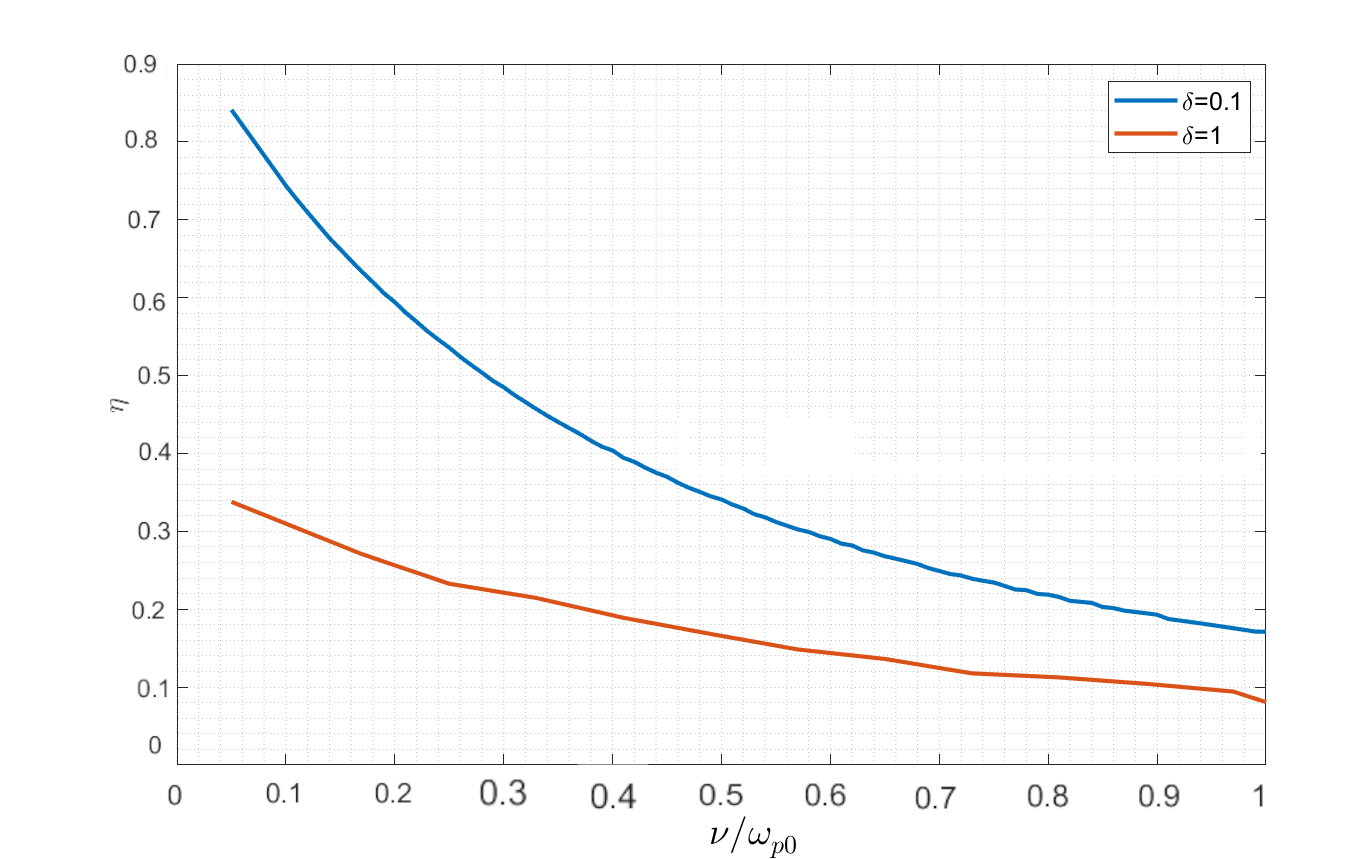
\includegraphics[width=1\linewidth]{pics/kpd_nu}
	\caption{Эффективность излучения в зависимости от частоты соударений $\nu/\omega_{p0}$ \\при разных размерах неоднородной области $\delta$.}
	\label{ris:kpd_nu}
\end{figure}